\documentclass[12pt, a4paper]{article}

\usepackage{setspace, graphicx, lineno, caption, color, float}
\usepackage{amsmath}
\usepackage{amsfonts}
\usepackage{amssymb}
\usepackage{amsthm}
\usepackage{amstext} %to enter text in mathematical formulae
\usepackage[retainorgcmds]{IEEEtrantools}
\usepackage{natbib}
\usepackage{hyperref} % for linking refferences to supps

%page set up
\usepackage[left=2.5cm,top=2.5cm,right=2.5cm, bottom=2.5cm,nohead]{geometry}

%paragraph formatting
\setlength{\parskip}{12pt}
\setlength{\parindent}{0cm}

\setcounter{figure}{0}
\renewcommand{\thefigure}{S\arabic{figure}}

\begin{document}
\section*{Appendix 5: Finding which initial conditions and model parameters lead to which IPM strategies}
It is unlikely a given IPM strategy will perform well in all scenarios, for example strategy that works well in cases where the yield penalty ($Y_D$) of the weed is very low is unlikely to be good in cases where the yield penalty is very high. To find the parameters and initial conditions ($n_0$) that most influence what makes a good IPM strategy we extend the meta-modelling approach outlined in \citep{Cout2014} to complex multivariate time series outputs (i.e. the sequences of the four sub actions). The meta-modelling approach to global sensitivity analysis is very flexible, and only requires building a function that predicts a models output given a set of parameters. The complication in this case is that the model output is a time series of actions, rather than a single number. To address this we carry out the sensitivity analysis as follows:
\begin{enumerate}
\item We use latin hypercube sampling to generate 15000 parameter combinations. We treat the initial conditions as parameters ($Rr_\text{int}$, $Qq_\text{int}$ and $N_\text{int}$). 
\item For each parameter combination we run the genetic algorithm (\nameref{app:GA}) for 100 iterations, experience showed that improvements to the best solution found dramatically slowed down after 60 iterations with a solution set size of 100 and mutation rate or 0.03. After 100 iterations we choose the action sequence with the highest reward as the best action sequence.     
\item This resulted in 15000 action sequences. We only use the first 10 time steps of each action sequence, although the reward was calculated over 25 time steps. This ensured that the action chosen at each time step was done so considering rewards from at least 15 time steps in to the future. To make sense of this mass of data we organised these action sequences by finding how they differed in relation to one another. The first step in this process was to build a dissimilarity matrix of each action sequence to all the other action sequences. We use a distance metric from text analysis, longest common sub-sequence, calculated with the 'SimilarityMeasures' \citep{Tooh2015} package in R. We allow a positional displacement of one time step, that is actions in sequence 1 are allowed to be matched to actions in sequence 2 that are separated in time by at most one time step. This allows out of phase cycles to have very high similarity. Two action sequences where the same combinations of actions are used, but at different times will have low similarity. We use non-metric multi-dimensional scaling (NMDS), implemented with the 'ecodist' package \citep{Gosl2007} to project this very high dimensional dissimilarity matrix into a lower dimensional space. We call this the solution space and we found that we could project the dissimilarity matrix into an eight dimensional solution space, with a stress of 0.09. Stress measures the difference between the relative location of each solution in the solution space, and the dissimilarity matrix lower values are better. We found that 8 dimensions was a good trade-off between low stress and a manageable number of dimensions. Figure \ref{fig:clust_NMDS} shows how the matches up to a separate hierarchical clustering (using the wardD2 method) we carried out to confirm and aid visualisation of the NMDS.                  
\item We recorded the eight co-ordinates of each solution in the solution space, along with the parameter set that generated that solution. This built a dataset 15000 rows long, where each row was a parameter set and a location in the solution space.
\item We use multi-variate boosted regression trees (mvBRT) as our meta-model. mvBRTs were fit using the 'mvtboost' package \citep{Mill2016}. mvBRTs fit a separate boosted regression tree to each dimension of the response, in our case the eight dimensional solution space. At each iteration in each tree the split that most reduced the co-variance between responses is choose. For further details see \citep{Mill2016}. We used a learning rate of 0.01, maximum interaction depth of 5. These tuning parameters lead to a optimum of 12229 trees in each BRT.
\item We interrogate the mvBRT to find the most influential parameters. We also calculate partial dependence plots of the mvBRT to predict where in the solution space a given set of parameters leads to, and use the closest solution to that location to estimate what a solution in the predicted location would look like. We use this as guide to help us explore and and interrogate the complex solution space. However, we have access to the data generating process and so do not need to rely on this estimate. For the actual plots in the results we re-run the genetic algorithm with the desired parameter combinations.                  
\end{enumerate}       

\begin{figure}[!h]
	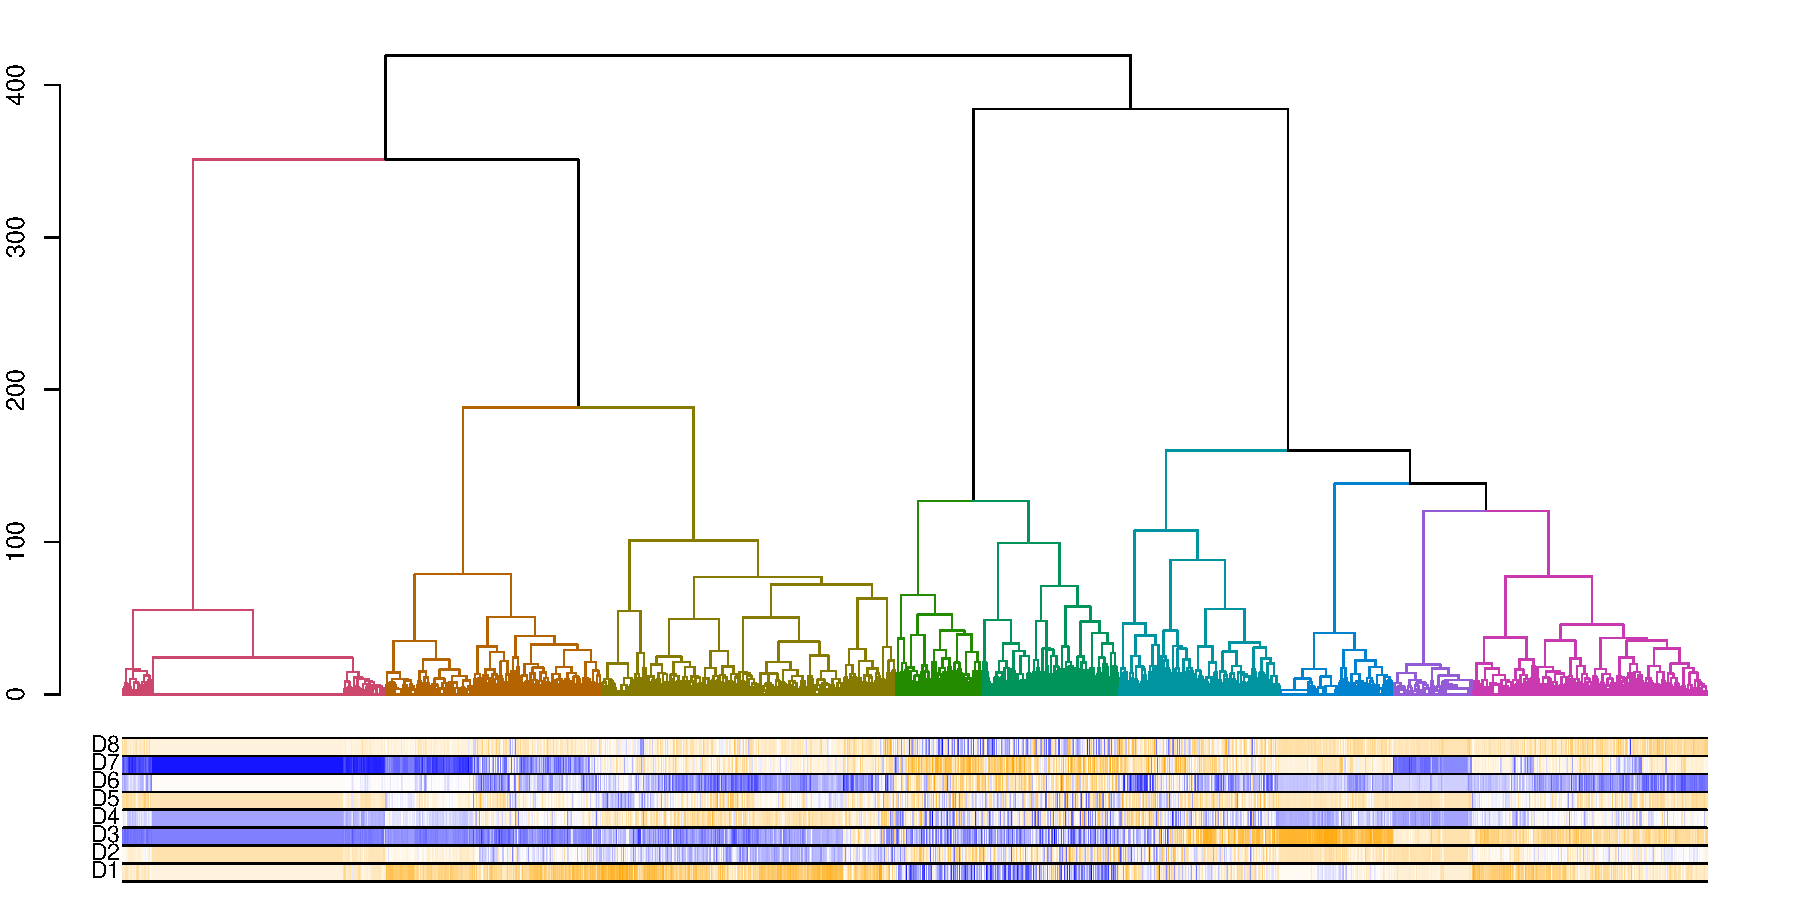
\includegraphics[width=170mm]{MS_figs/dend_9clust_NMDS_8D.pdf}
	\caption{Position of all 15000 IPM strategies found by the genetic algorithm in the eight dimensional solution space and dendrogram built using the wardD2 method. Different colours in the dendrogram highlight the 9 most distinct clusters. Colours in the bars show each solutions position in the solution space. All dimensions are centred on 0 (white), with dark blues being at one extreme and dark oranges a the other (only relative position is meaningful).} 
	\label{fig:clust_NMDS}
\end{figure}

\paragraph*{Appendix 3}
\label{app:GA}
Genetic Algorithm

\bibliographystyle{/Users/shauncoutts/Dropbox/shauns_paper/referencing/bes}
\bibliography{/Users/shauncoutts/Dropbox/shauns_paper/referencing/refs} 

\end{document}
